\subsection{Sequence Diagram}

Here reported the sequence diagram for the requesting a person from database. The user executes a GET request to the web server, specifying the URI /movie-webapp-1.00/get-person. Additionally, the data about the person which is trying to retrieve information (personID) is passed to the web server. The web server instantiates the GetPersonServlet and calls its doGet() method, passing the HttpServletRequest and the HttpServletResponse. Given the GET data, it is searching a person inside the database with person ID data. The control is passed to the GetPersonByIdDAO which receives as an argument the connection (defined in AbstractDatabaseServlet extended by the GetPersonServlet) and searched the person. The GetPersonByIdDAO extends the AbstractDAO and contacts the Database Serverwhich executes the SQL statement for searching a person. This DAO return the personal information about the person. To collect all the information about the person, GetPersonServlet performs two other Database access operations; GetAwardsAndMovieNameByPersonIdDAO and GetMoviesByPersonIdDAO. The purpose of these operations is to collect all the information about the person including movies which s/he participated and awards which s/he won. If some errors occur, the control is returned to the GetPersonServlet and a new String object contains the relevant situation is created. Finally, the person found in the database is returned to the user with all the information about the person. 


\bigskip

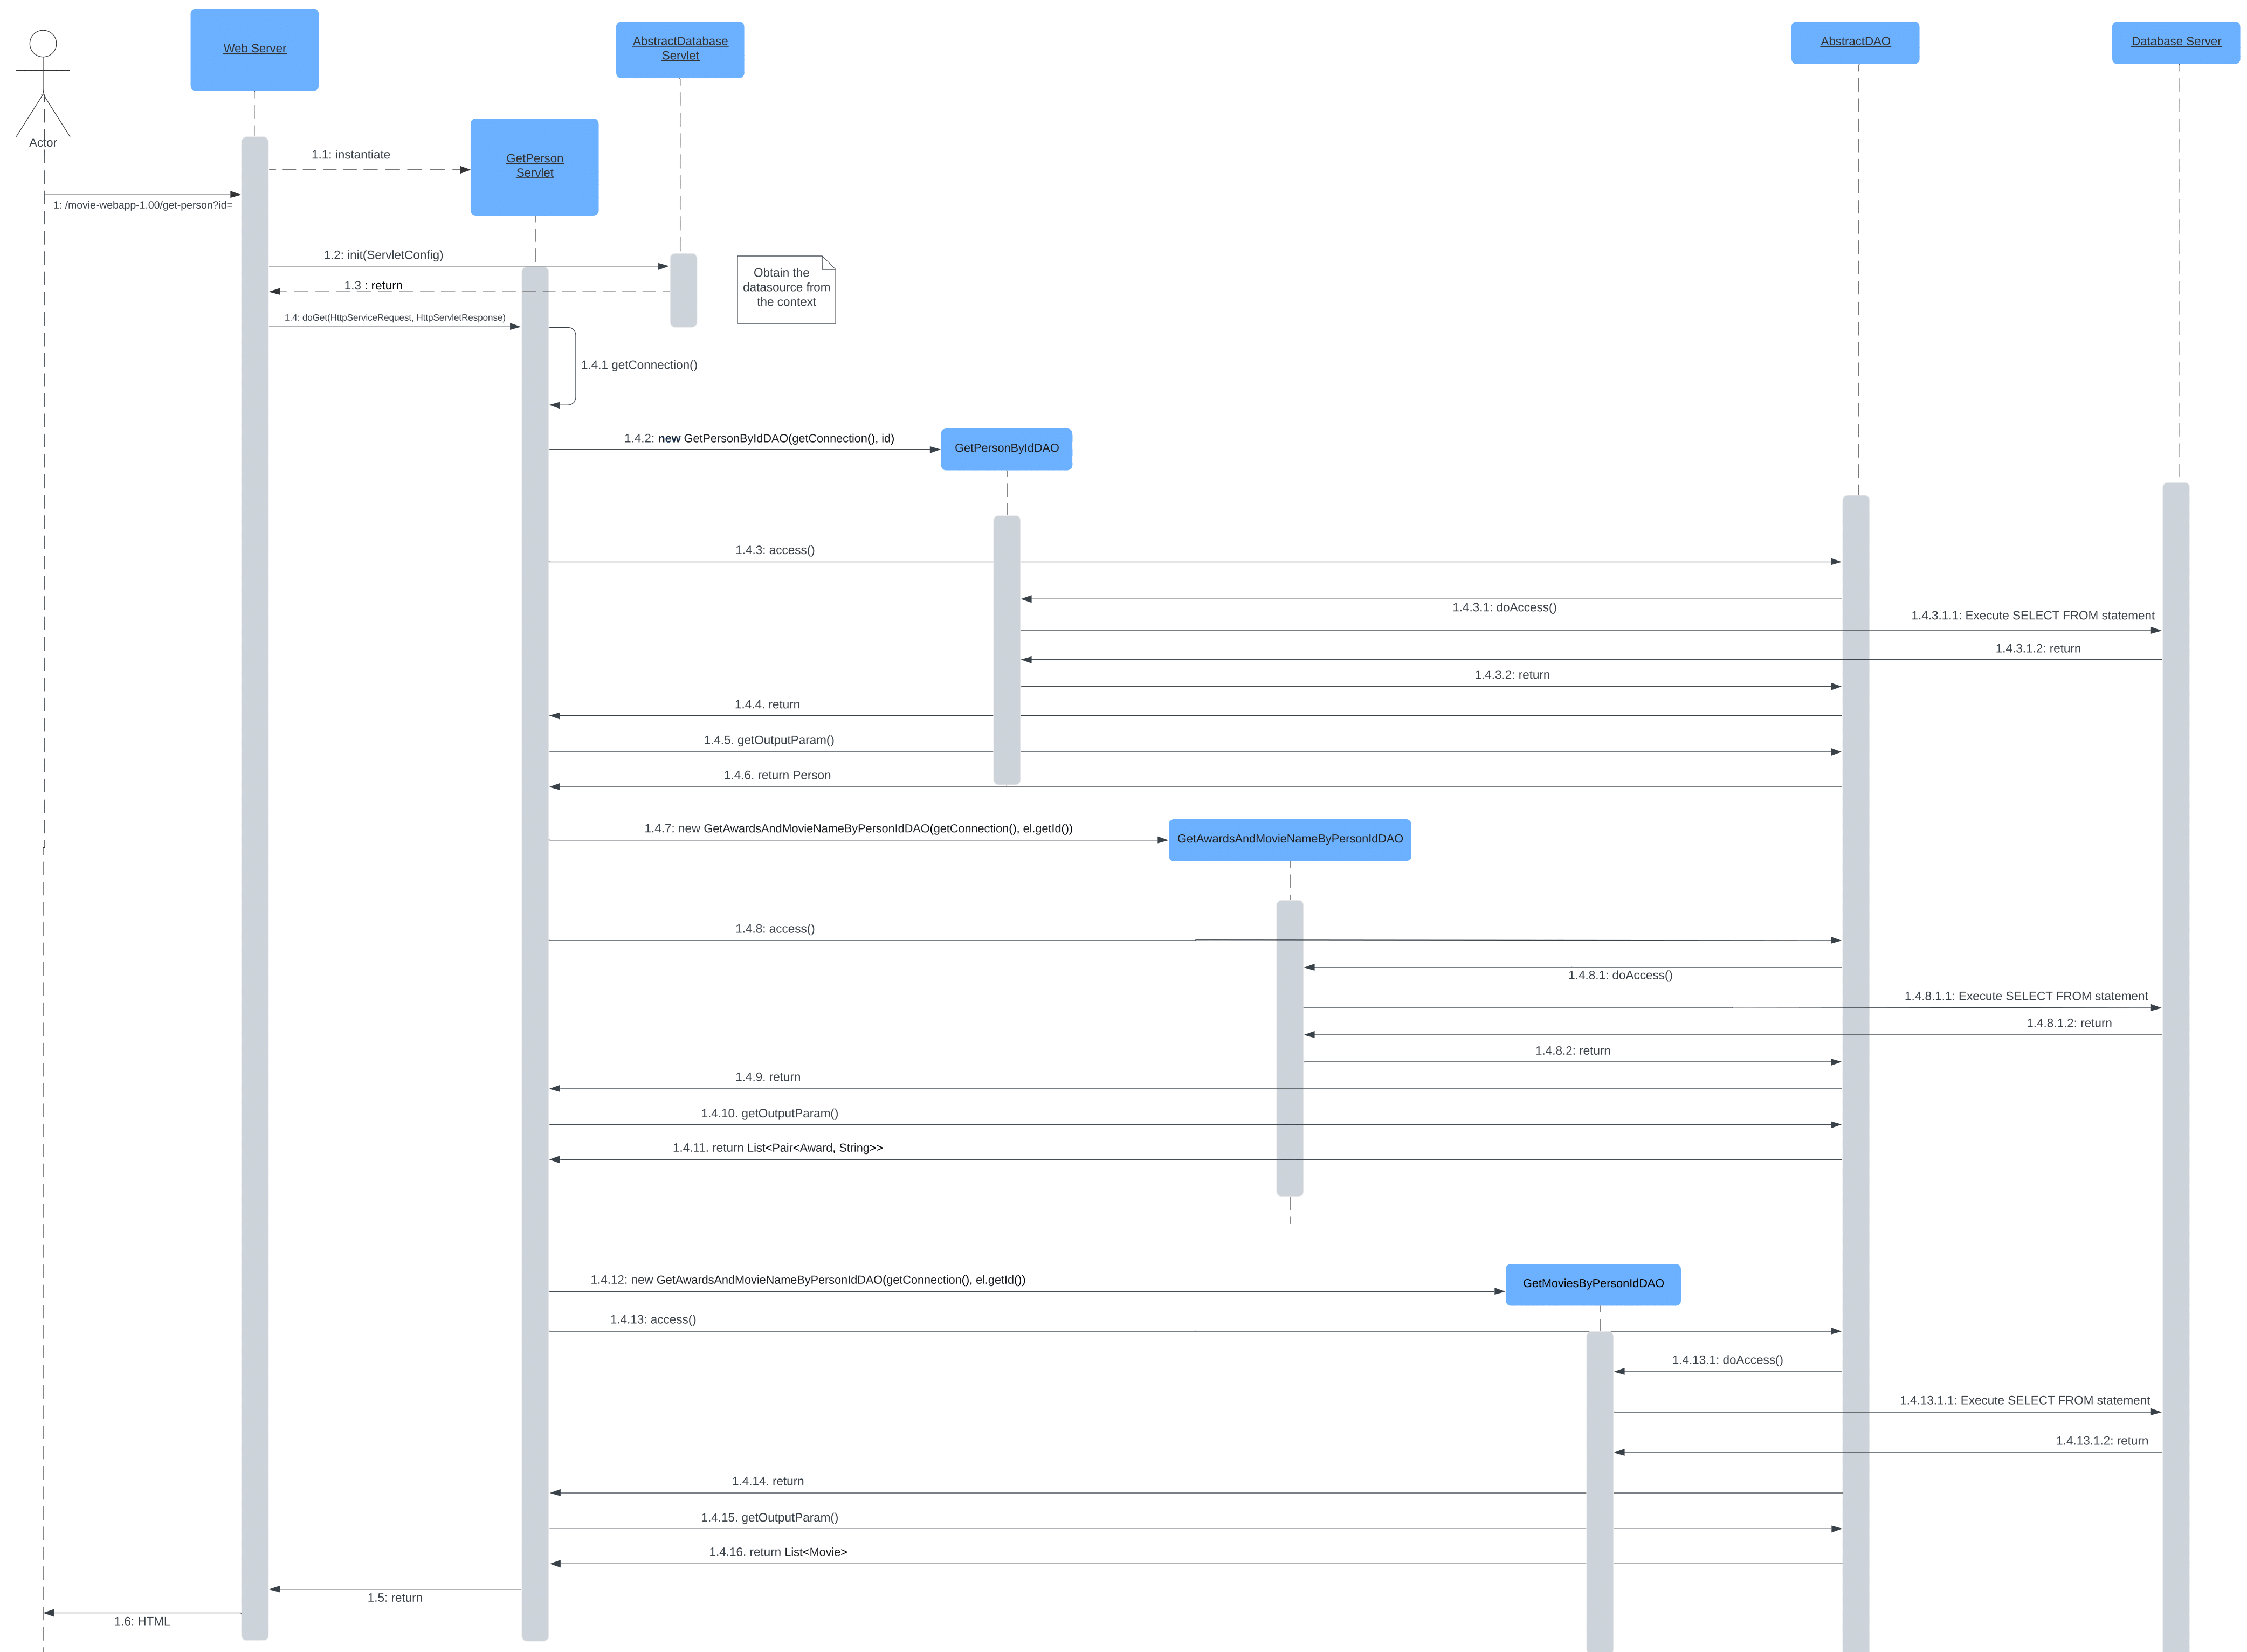
\includegraphics[angle=90, width=0.85\textwidth]{pictures/GetPersonServlet-1.png}

%describe here the sequence diagram